\documentclass[12pt]{article}
\usepackage{amsmath}
\usepackage{graphicx}
\usepackage{hyperref}
\usepackage[latin1]{inputenc}
\usepackage{float}
\usepackage[a4paper, portrait, margin=0.5in]{geometry}

\graphicspath{ {./img/} }

\title{CS547 Assignment 3\\Multi-Objective Optimisation}
\author{Wojciech Cichoradzki\\201506554}
\date{14/11/2019}

\begin{document}
\maketitle

\section{Results}

\begin{figure}[H]
  \centering
  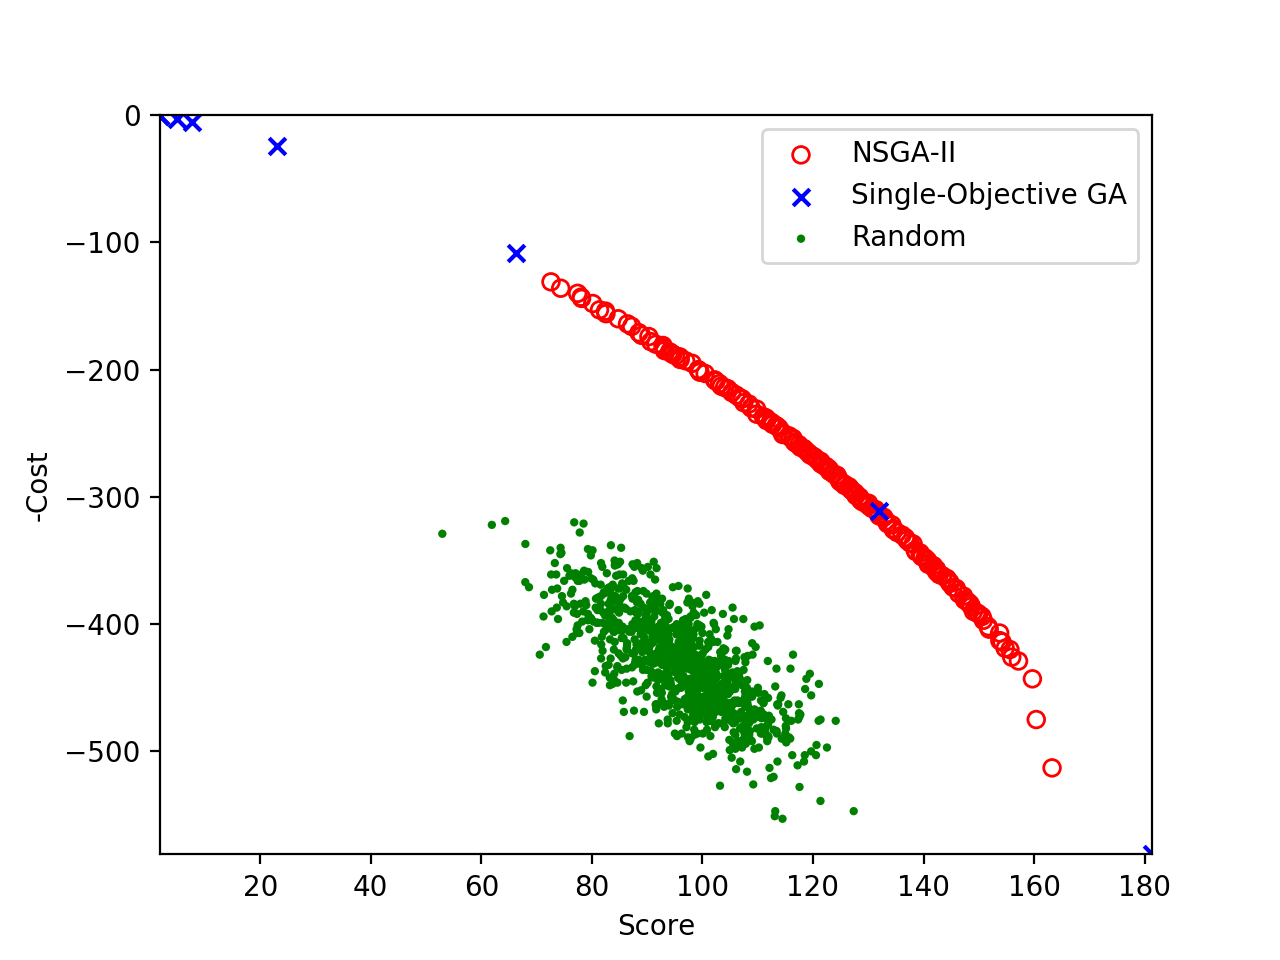
\includegraphics[width=0.49\textwidth]{classic_no_constraint}
  \caption{Unconstrained budget, classic/nrp1 dataset, population 200, 15 000 runs}
  \label{fig:1}
\end{figure}

\begin{figure}[H]
  \centering
  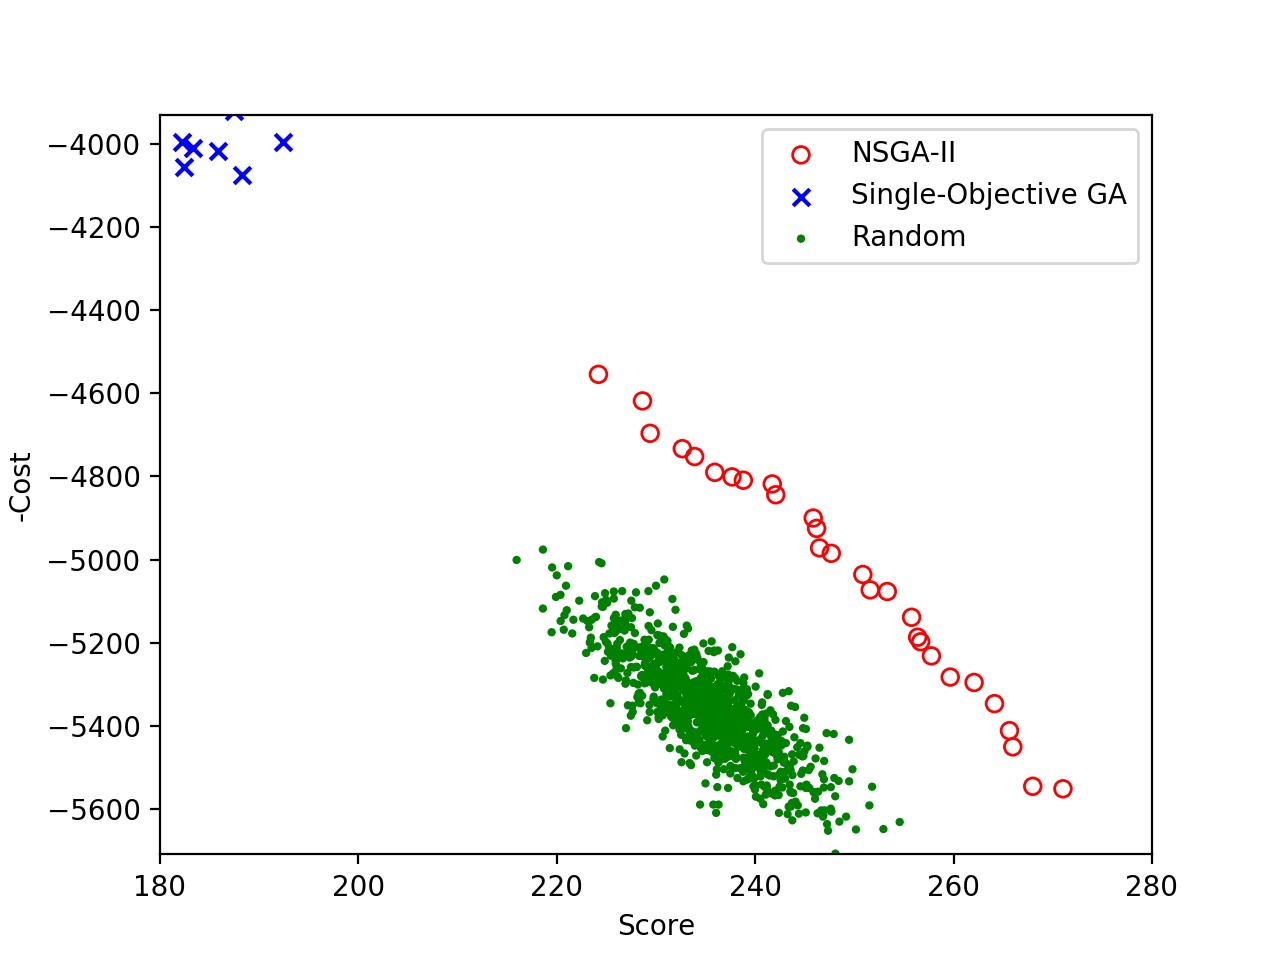
\includegraphics[width=0.49\textwidth]{realistic_no_constraint}
  \caption{Unconstrained budget, realistic/nrp-g4 dataset, population 100, 2000 runs}
  \label{fig:2}
\end{figure}

\begin{figure}[H]
  \centering
  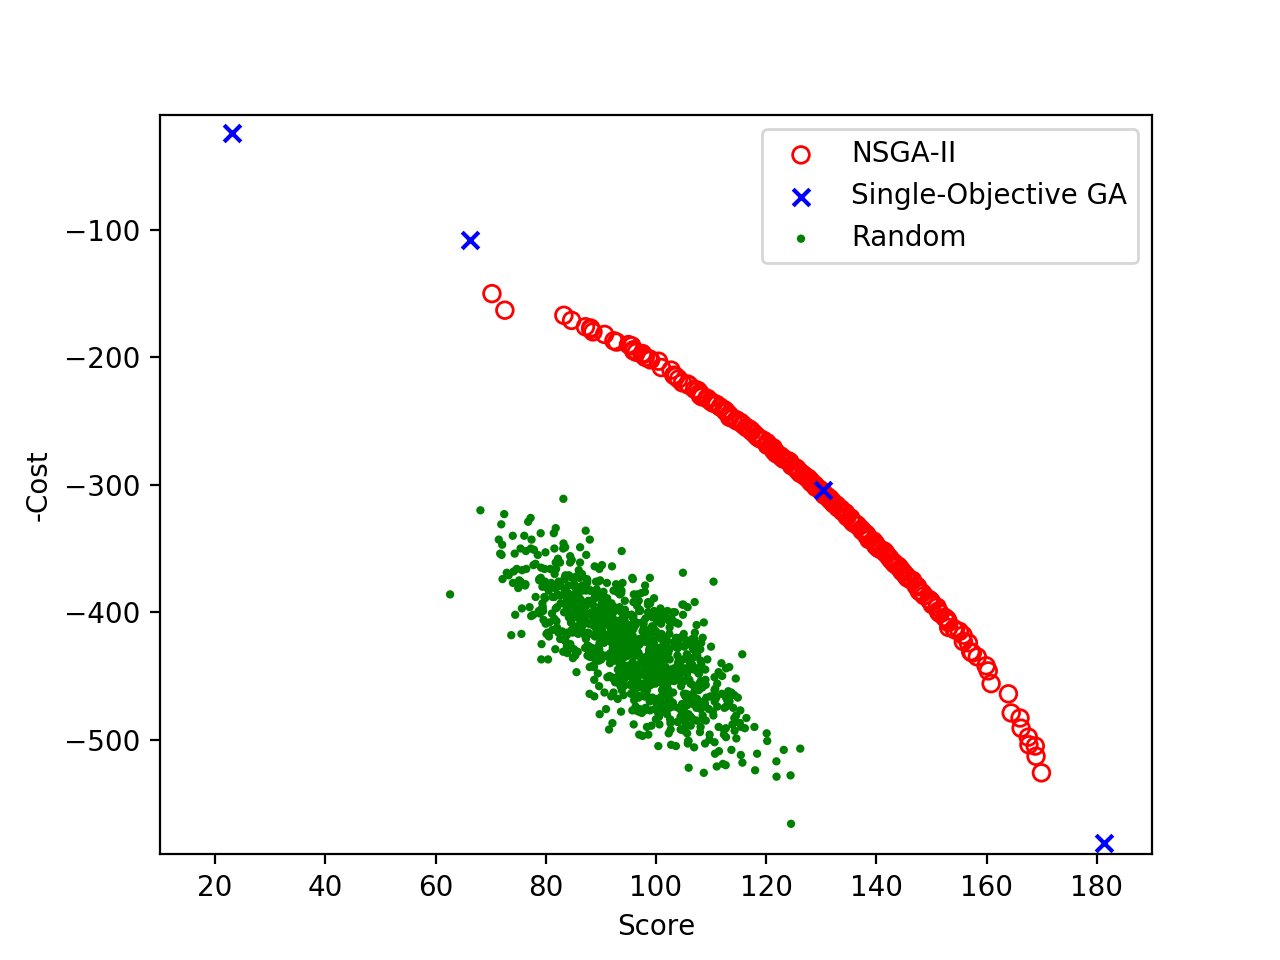
\includegraphics[width=0.49\textwidth]{classic_constraint}
  \caption{Constrained budget, classic/nrp1 dataset, population 200, 15 000 runs}
  \label{fig:3}
\end{figure}

\begin{figure}[H]
  \centering
  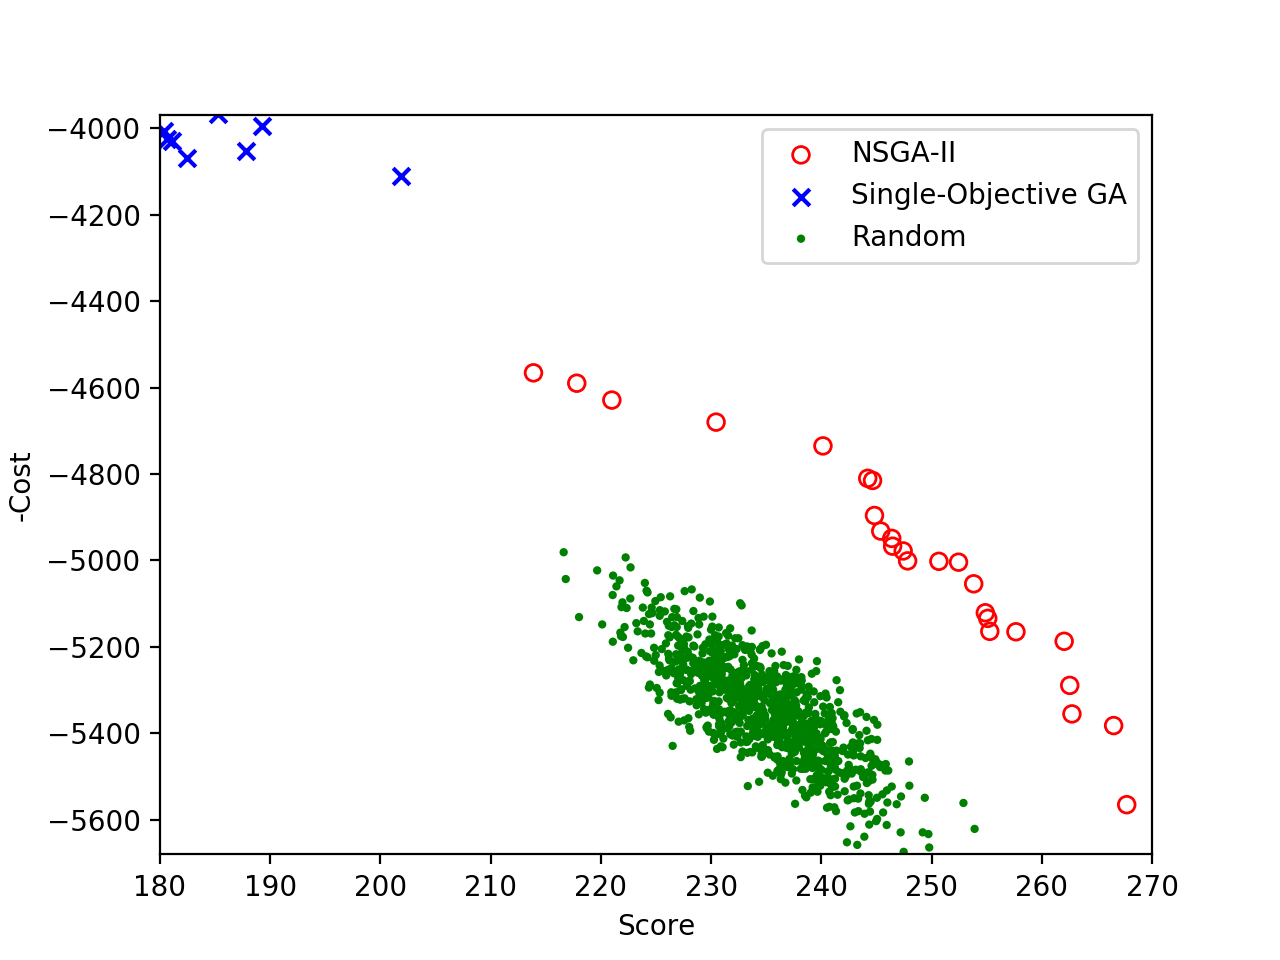
\includegraphics[width=0.49\textwidth]{realistic_constraint}
  \caption{Constrained budget, realistic/nrp-g4 dataset, population 100, 2000 runs}
  \label{fig:4}
\end{figure}

\section{Algorithm}
The case study compares two different evolutionary algorithms to random search: NSGA-II and a single-objective GA. The single-objective GA is implemented as in the relevant section of the "Techniques, Taxonomy, tutorial" paper with the 9 different weights applied ranging from 0.1 to 0.9 with 0.1 step. Two different datasets were used for evaluation - classic/nrp1 dataset with 140 requirements and 100 customers and realistic/nrp-g4 dataset with 2246 requirements and 294 customers. Classic dataset was used with population of 200 and run 15000 generations, while the realistic one used population of 100 and run for 2000 generations. Classic dataset required much less time to compute all algorithm, taking less than 10 minutes to finish, while the realistic was CPU and memory expensive and took more than an hour to finish with half the population and significantly less runs. Both dataset were also tested against constrained and unconstrained budget - constraint was set to half the total cost of all requirements. Customers weightings were modified from the provided by dataset by taking fraction of given score to total score of all customers so the sum of scores add up to 1 (with floating-point precision error).
\newpage
Weights of the requirements were assigned using the provided order using the simple formula:
\[ \frac{N-n}{N} * 100 \]
,where \(N = \)number of all user requirements, and \( n = \)0-based requirement index e.g. first requirement out of 4 would have weight of:
\[ \frac{4-0}{4} * 100 = 100 \]
,second:
\[ \frac{4-1}{4} * 100 = 75 \]
,third 50 and fourth 25. \\
Original, unchanged requirements numbers and costs were used. For all algorithms, additional constraint was introduced that rejected empty solutions (with no requirements satisfied) as it produced soltions with perfect cost score (0, obviously), but worst customer score (0, as well).
\section{Results}
All figures show that random search produces normally distributed solutions, whereas the weighted-sum, single-objective GA tends to produce solutions at the extremes of the Pareto front, especially for the larger dataset with less iterations (fig. \ref{fig:2}, fig.\ref{fig:4}). The Pareto front is dominantly produced by NSGA-II, forming the widest Pareto front that represts the trade-off between the cost and the expected profit, especially for smaller dataset (fig.\ref{fig:1}, fig.\ref{fig:3}). It is also clear that the Pareto front is better represented for smaller dataset, where the results are more optimised, producing steady curve in contrast to the larger dataset, where the curve produced tends to variate in its local derivative. Another observation is that with much smaller population size and less runs, tests on the larger dataset output results focused around different areas of the search space. Single-objective GA tend to occupy solutions with low cost and low score, whilst the NSGA-II solutions on larger dataset tend to be slightly more focused around lower-right part of the graph compared to wider-to-the-left space in terms of smaller dataset. This, however might be just beacuse of the flaw with not enough iterations and smaller population size. There is not much difference between constrained and unconstrained problem definition, as the budget constraint should have probably be set to smaller value as it was not causing any differences in the results (it was additional, out of scope of the exercise additional test anyway).

\section{Running the package}
In the root of the project run:\\
\texttt{python3 -m next\_release\_problem.start -c <config\_file.json>}\\
For example:\\
\texttt{python3 -m next\_release\_problem.start -c config-classic-constrained.json}\\
Runs the genetic algorithm config using the small data set.

\end{document}
